\documentclass[margin=1in]{article}
\usepackage[utf8]{inputenc}
\usepackage[english]{babel}
\usepackage{amsmath}
\usepackage{graphicx}
\usepackage{capt-of}
\usepackage{lipsum}
\usepackage{graphicx}
\usepackage{listings}
\usepackage{xcolor} % For custom colors
\lstset{
	language=R,                % Choose the language (e.g., Python, C, R)
	basicstyle=\ttfamily\small, % Font size and type
	keywordstyle=\color{blue},  % Keywords color
	commentstyle=\color{gray},  % Comments color
	stringstyle=\color{red},    % String color
	numbers=left,               % Line numbers
	numberstyle=\tiny\color{gray}, % Line number style
	stepnumber=1,               % Numbering step
	breaklines=true,            % Auto line break
	backgroundcolor=\color{black!5}, % Light gray background
	frame=single,               % Frame around the code
}
\usepackage{float}
\usepackage[margin=1in]{geometry}
\usepackage[]{amsthm} %lets us use \begin{proof}
		\usepackage[]{amssymb} %gives us the character \varnothing
		
	
	
	\title{Homework 1, MATH 5010}
	\author{Zongyi Liu}
	\date{Feb 11, 2025}
	\begin{document}
		\maketitle
		
		\subsubsection*{Question 0}
		Some of the pictures in this file go down to succeeding pages, and I tried to adjusted them with \texttt{pagebreak} or such syntax, but the formatting were not successful, please do not deduct points because of this. Thank you.
		
		\subsubsection*{Question 1}
		 Suppose that the spot rate of EUR is 1.02395 USD for 1 Euro. 1 year forward rate is 1.06280 USD for 1 Euro. Suppose that the 1 year USD interest rate is $4.21 \%$ annualized and Euro interest rate is $2.38 \%$ annualized. Rates are compounded annually that means that 1 USD a year from now grows to $1^{*}(1+0.0421)$ USD. Is there an arbitrage opportunity? If there is, describe it (what you borrow, what you invest etc.)
		 
		 \textbf{Answer}
		 
		 This year, $1.02395\ USD = 1\ Euro$, with the annualized interest rate given to both currencies, we can compute as $1.02395\cdot(1+0.0421)\ USD=1\cdot(1+0.0238)\ Euro$, and the theoretical 1 year forward rate is  $\frac{\left(1.02395\cdot\left(1+0.0421\right)\right)}{1\cdot\left(1+0.0238\right)}=1.042252681$, which is smaller than the 1-year forward rate of $1.06280$. Thus there is an arbitrage opportunity.
		 
		 \begin{itemize}
		 \item Sell 1 year forward 1 Euro at \$1.06280 per Euro
		 \item Borrow \$1.0001465 = \$1.02395/(1+2.38\%) at 4.21\%. Here we have to repay \$1.02395*(1+4.21\%)/(1+2.38\%)=\$1.04225 in 1 year
		 \item Exchange\$ 1.0001465 at a spot rate \$1.02395=1 Euro. Get 1/(1+2.38\%)= 0.97675 Euro now.
		 \item Deposit 0.97675 Euro now at 2.38\% for 1 year. Get 1 Euro in 1 year.
		 \item In 1 year using forward that we entered exchange, and here we have 1 Euro into \$1.06280; repay \$1.04225 that we have to repay
		 \item Profit in 1 year 1.06280-1.04225= \$0.02055
		 \end{itemize}
		 
		 \pagebreak
		 
		 \subsubsection*{Question 2}
		 Suppose that the spot exchange rate of EUR is 1.0240 USD for 1Euro. Suppose that the 3 months USD interest rate is $4.30 \%$ annualized and Euro interest rate is $2.59 \%$ annualized (now rates that used here are continuously compounded). What is the 3 month forward exchange rate?
		 
		 \textbf{Answer}
		 
		 The timespan here is $3/12=\frac{1}{4}\ Year$, so we have
		 
		 \begin{itemize}
		 	\item $1.024\cdot e^{\left(1.043\cdot0.25\right)}=1.3290528$
		 	\item $1\cdot e^{\left(1.0259\cdot0.25\right)} = 1.29236$
		 \end{itemize}
	 
	 And thus the 3 month forward exchange rate is $\frac{1.329052825}{1.292366456}=1.028387$
		 
		 
		 \subsubsection*{Question 3}
		 What does it mean for interest rate to be negative? Read the document from courseworks. Explain in 4 lines.
		  
		  \textbf{Answer}
		  
		  Negative interest rates mean banks pay to hold reserves at central banks instead of earning interest. This policy, used by the ECB and Bank of Japan, aims to boost lending and weaken the currency. It pushes down short-term interest rates, affecting loans and investments. However, its effectiveness is uncertain, and it poses challenges for banks and depositors.
		  

		  \subsubsection*{Question 4}
		  What is the six-month forward price for a stock providing no income. The stock price is 100 and the continuously compounded interest rate is $4 \%$? What is the forward price if the stock pays a $3 \%, 4 \%, 5 \%$ continuously compounded dividend yield?
		  
		  \textbf{Answer}
		  
		  The six-month forward price providing no income is
		  
		  $100*e^{((4\%-0)(6/12))}=102.020134$
		  
		  If the stock pays $3\%$
		  
		  $100*e^{((4\%-3\%)(6/12))}=100.5012521$
		  
		   If the stock pays $4\%$
		  
		  $100*e^{((4\%-4\%)(6/12))}=100$
		  
		   If the stock pays $5\%$
		  
		  $100*e^{((4\%-5\%)(6/12))}=99.50124792$
		  
		   \pagebreak
		  \subsubsection*{Question 5}
		  What is the difference between a forward contract and a futures contract?
		  
		  \textbf{Answer}
		  
		  The \textbf{forward contracts} is a custom-made agreements between two parties to buy or sell an asset at a specific price on a future date. It is a non-standardized contract between two parties to buy or sell an asset at a specified future time at a price agreed on in the contract; it is a type of derivative instrument. The party agreeing to buy the underlying asset in the future assumes a long position, and the party agreeing to sell the asset in the future assumes a short position. The price that both sides agree upon is called \textbf{delivery price} (as quoted in class slides).
		  
		  Whereas the \textbf{futures contracts} is standardized contracts with set quantities, qualities, and delivery dates. It is a standardized legal contract to buy or sell something at a predetermined price for delivery at a specified time in the future. The predetermined price of the contract is known as the \textbf{forward price} or \textbf{delivery price} (the name of the term is same as the price for forward contracts, as quoted from Wikipedia). The specified time in the future when delivery and payment occur is known as the \textbf{delivery date}. The futures typically traded in future exchange and settled daily, whereas forward contracts don't have specific places to make deal. Thus futures have far less counterparty risk as they guarantee payment on the agreed-upon date, and futures contracts have greater flexibility and liquidity than forward contacts.
		  
		  We can come up with a table to illustrate.
		  
		  \begin{table}[h!]
		  	\caption{Differences Between Futures Contracts and Forward Contracts}
		  	\centering
		  	\small % Reduce font size
		  	\setlength{\tabcolsep}{4pt} % Reduce column padding
		  	\begin{tabular}{|p{0.25\textwidth}|p{0.35\textwidth}|p{0.35\textwidth}|}
		  		\hline
		  		\textbf{Features} & \textbf{Futures Contract} & \textbf{Forward Contract} \\ \hline
		  		\textbf{Trading Venue} & Traded on organized exchanges (e.g., CME, NYMEX). & Traded over-the-counter (OTC), privately negotiated between parties. \\ \hline
		  		\textbf{Standardization} & Highly standardized (contract size, expiration date, and terms are fixed). & Customizable to meet the specific needs of the parties involved. \\ \hline
		  		\textbf{Liquidity} & More liquid due to exchange trading and standardization. & Less liquid, as they are tailored and not easily transferable. \\ \hline
		  		\textbf{Counterparty Risk} & Low, as the exchange acts as the counterparty and guarantees the contract. & Higher, as there is no intermediary; risk depends on the creditworthiness of the parties. \\ \hline
		  		\textbf{Settlement} & Daily settlement (marked-to-market). & Settled at the end of the contract term. \\ \hline
		  		\textbf{Regulation} & Heavily regulated by exchanges and government authorities. & Less regulated, as they are private agreements. \\ \hline
		  		\textbf{Contract Size} & Fixed and standardized. & Flexible and negotiated between parties. \\ \hline
		  		\textbf{Maturity Date} & Fixed and standardized. & Flexible and negotiated between parties. \\ \hline
		  		\textbf{Cost} & May involve brokerage fees and margin requirements. & Typically no upfront costs, but may require collateral. \\ \hline
		  		\textbf{Purpose} & Often used for hedging and speculation by a wide range of market participants. & Primarily used for hedging by businesses or institutions with specific needs. \\ \hline
		  		\textbf{Transparency} & Prices and transactions are publicly available. & Prices and terms are private and not disclosed to the public. \\ \hline
		  		\textbf{Delivery} & Rarely results in physical delivery; most contracts are closed before expiration. & Often results in physical delivery of the underlying asset. \\ \hline
		  	\end{tabular}
		  	
		  	\label{tab:futures_vs_forwards}
		  \end{table}
		  \pagebreak
		  
		  \subsubsection*{Question 6}
		  Make futures margin table similar to the class handout using oil futures prices spreadsheet \texttt{Oil CLH25.xls} on courseworks. Suppose that initial margin is 5,720 USD and a maintenance margin 5,200 USD per contract and margins are constant through the life of the contract. You buy 2 contracts at the close on September 13, 2023 and sell at the close on January 15,2025 . Oil futures point value is 1000\$. When are the margin calls?
		  
		  \textbf{Answer}
		  
		  In this excel, I firstly reverted the order of dates, and sorted the columns with dates increasing. Then calculate the \texttt{Daily gain}, \texttt{Cumulative Gain}, and \texttt{Margin Balance}. Margin calls happen when the margin balance is below the maintenance margin. The first margin call happens on Nov-7-2023, and then Jan-2-2024, Aug-5-2024, Sept-10-2024. On those days, we have \texttt{Marginal Balance} to be \$5152, \$5096, \$5150, and \$4986; all of them are below the maintenance margin, which is \$5200. 
		  
		  In the first margin call, we added \$568, and then add \$624, \$570, and \$734 in dates mentioned before. The final marginal balance is \$6789, and total cumulative gain is \$-1427. Testify by subtracting \$6789 by \$5720 and the sum of margin calls, which is \$2496. The result is \$-1427; it is the same amount as the total cumulative gain. 
		  
		  Moreover, this is for the single contract scenario, here we purchased 2 contracts, thus the result should multiply by 2, and the total cumulative gain is \$2854, and final marginal balance is \$13578.
		  
		  \begin{figure}[h]
		  	\caption{Last Several Rows of the Excel}
		  	\centering
		  	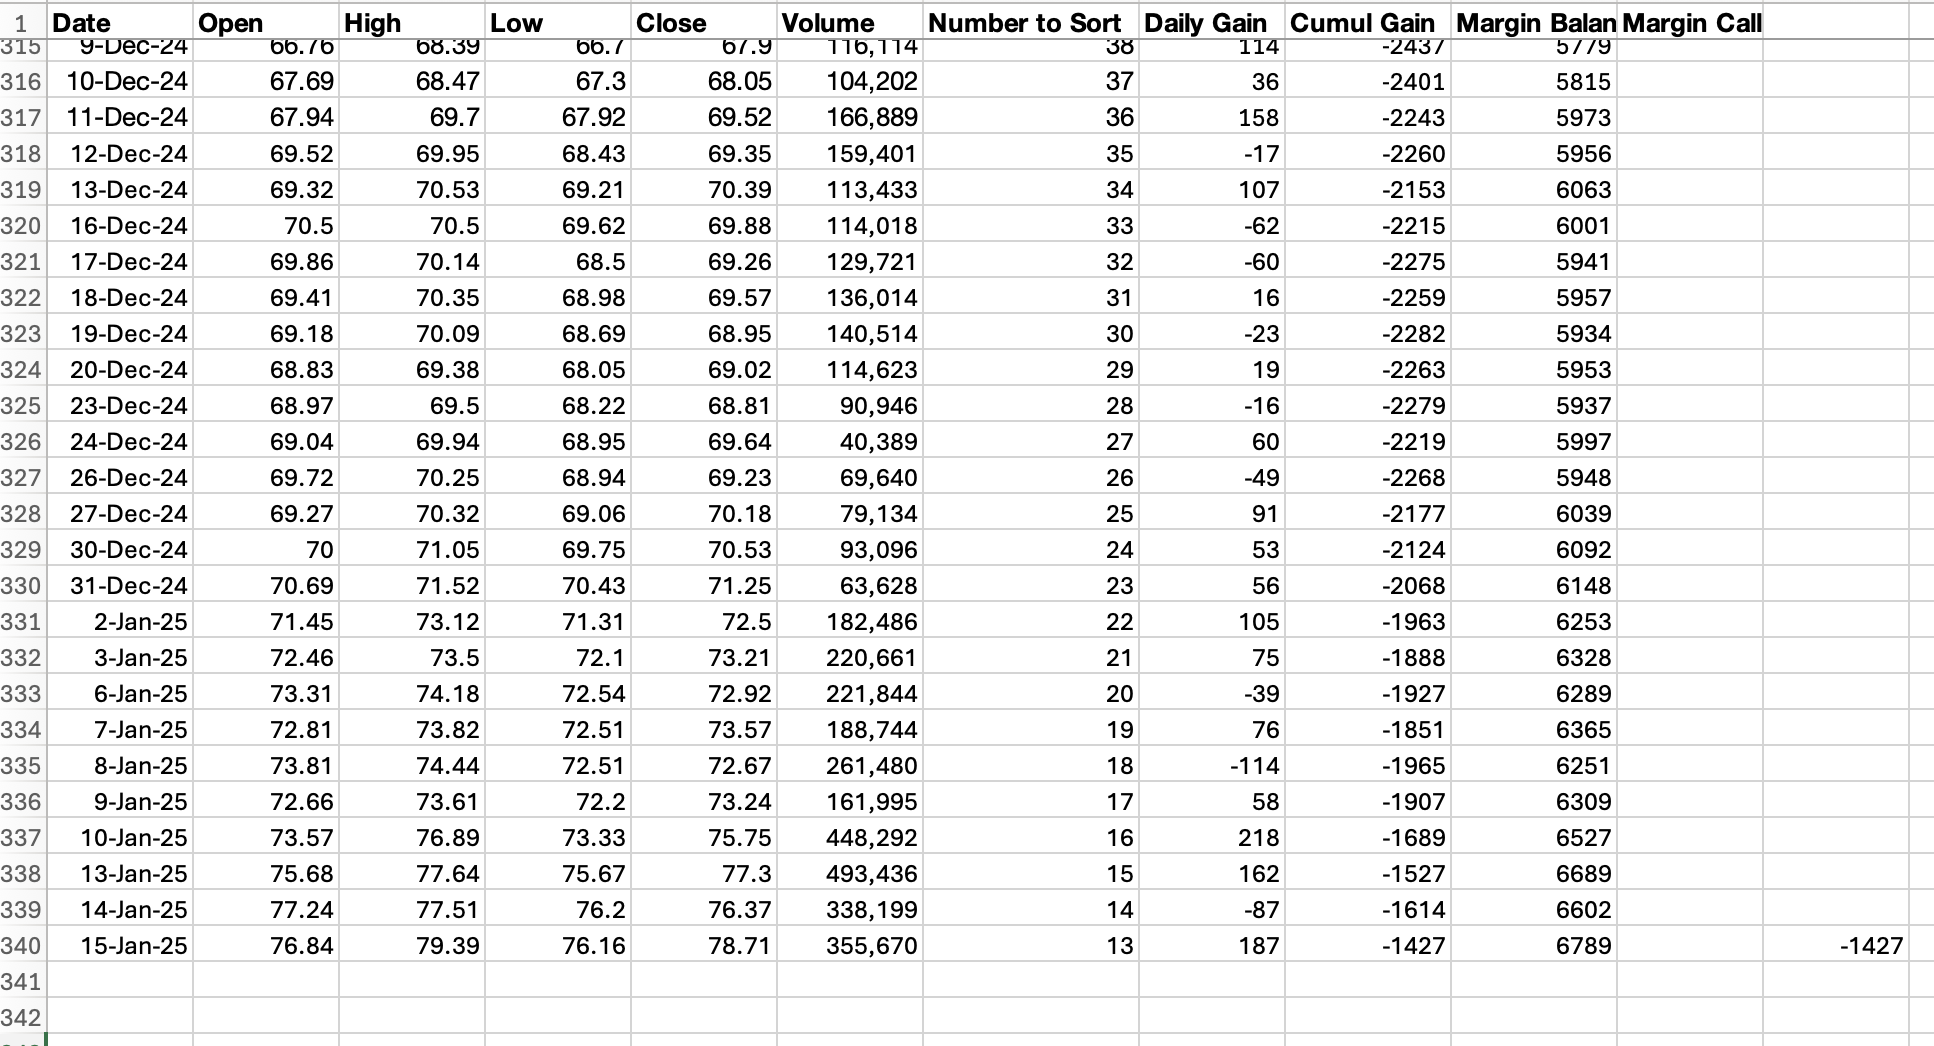
\includegraphics[width=0.7\textwidth]{HW1_Q6}
		  \end{figure}
		  
		   \pagebreak
		  \subsubsection*{Question 7}
		   This problem should be done in Excel and not in other programs. Go to http://finance.yahoo.com, chose Chart and type MSFT in the box. Click Historical Quotes below the chart. Input dates: Start January 24, 2014, End January 15, 2025. Click download spreadsheet format in the bottom of the page. Data is in the Excel format Date, Open, High, Low, Close, Volume, Adjusted Close. Make and submit the printouts of 2 plots: cumulative distribution functions of returns and approximate probability density function of returns using $0.2 \%$ horizontal intervals. Calculate mean, variance, standard deviation, mean absolute deviation, kurtosis and skewness of daily returns in Excel. You should use Excel and not other programs. If you need help with excel graphing talk to TAs. Use only adjusted close prices.
		   
		   \textbf{Answer}
		   
		   Firstly, to calculate the return, we need use the adjusted close price, with formula: $$Return=\frac{Adj\ Close_{t}-Adj\ Close_{t-1}}{Adj\ Close_{t-1}}$$
		   And in the excel, it implemented like \texttt{=(F3-F2)/F2} (suppose the adjusted close price is in column \texttt{F}, as defaultly set in the table when we downloaded it). After we get the return in column \texttt{H}, we need to round them into $0.02$, with the help of the function \texttt{=CEILING(H2,0.002)}, then to get the unique entry in the new column \texttt{=UNIQUE(I:I)}, and count their appearance with \texttt{=COUNTIF(I:I, J2)}. Finally, calculate their single probability with \texttt{=K3/COUNT(I:I)}. Then we can use the scatterplot in excel to get the probability density function plot.
		   \begin{figure}[h]
		   	\caption{Probability Density Function}
		   	\centering
		   	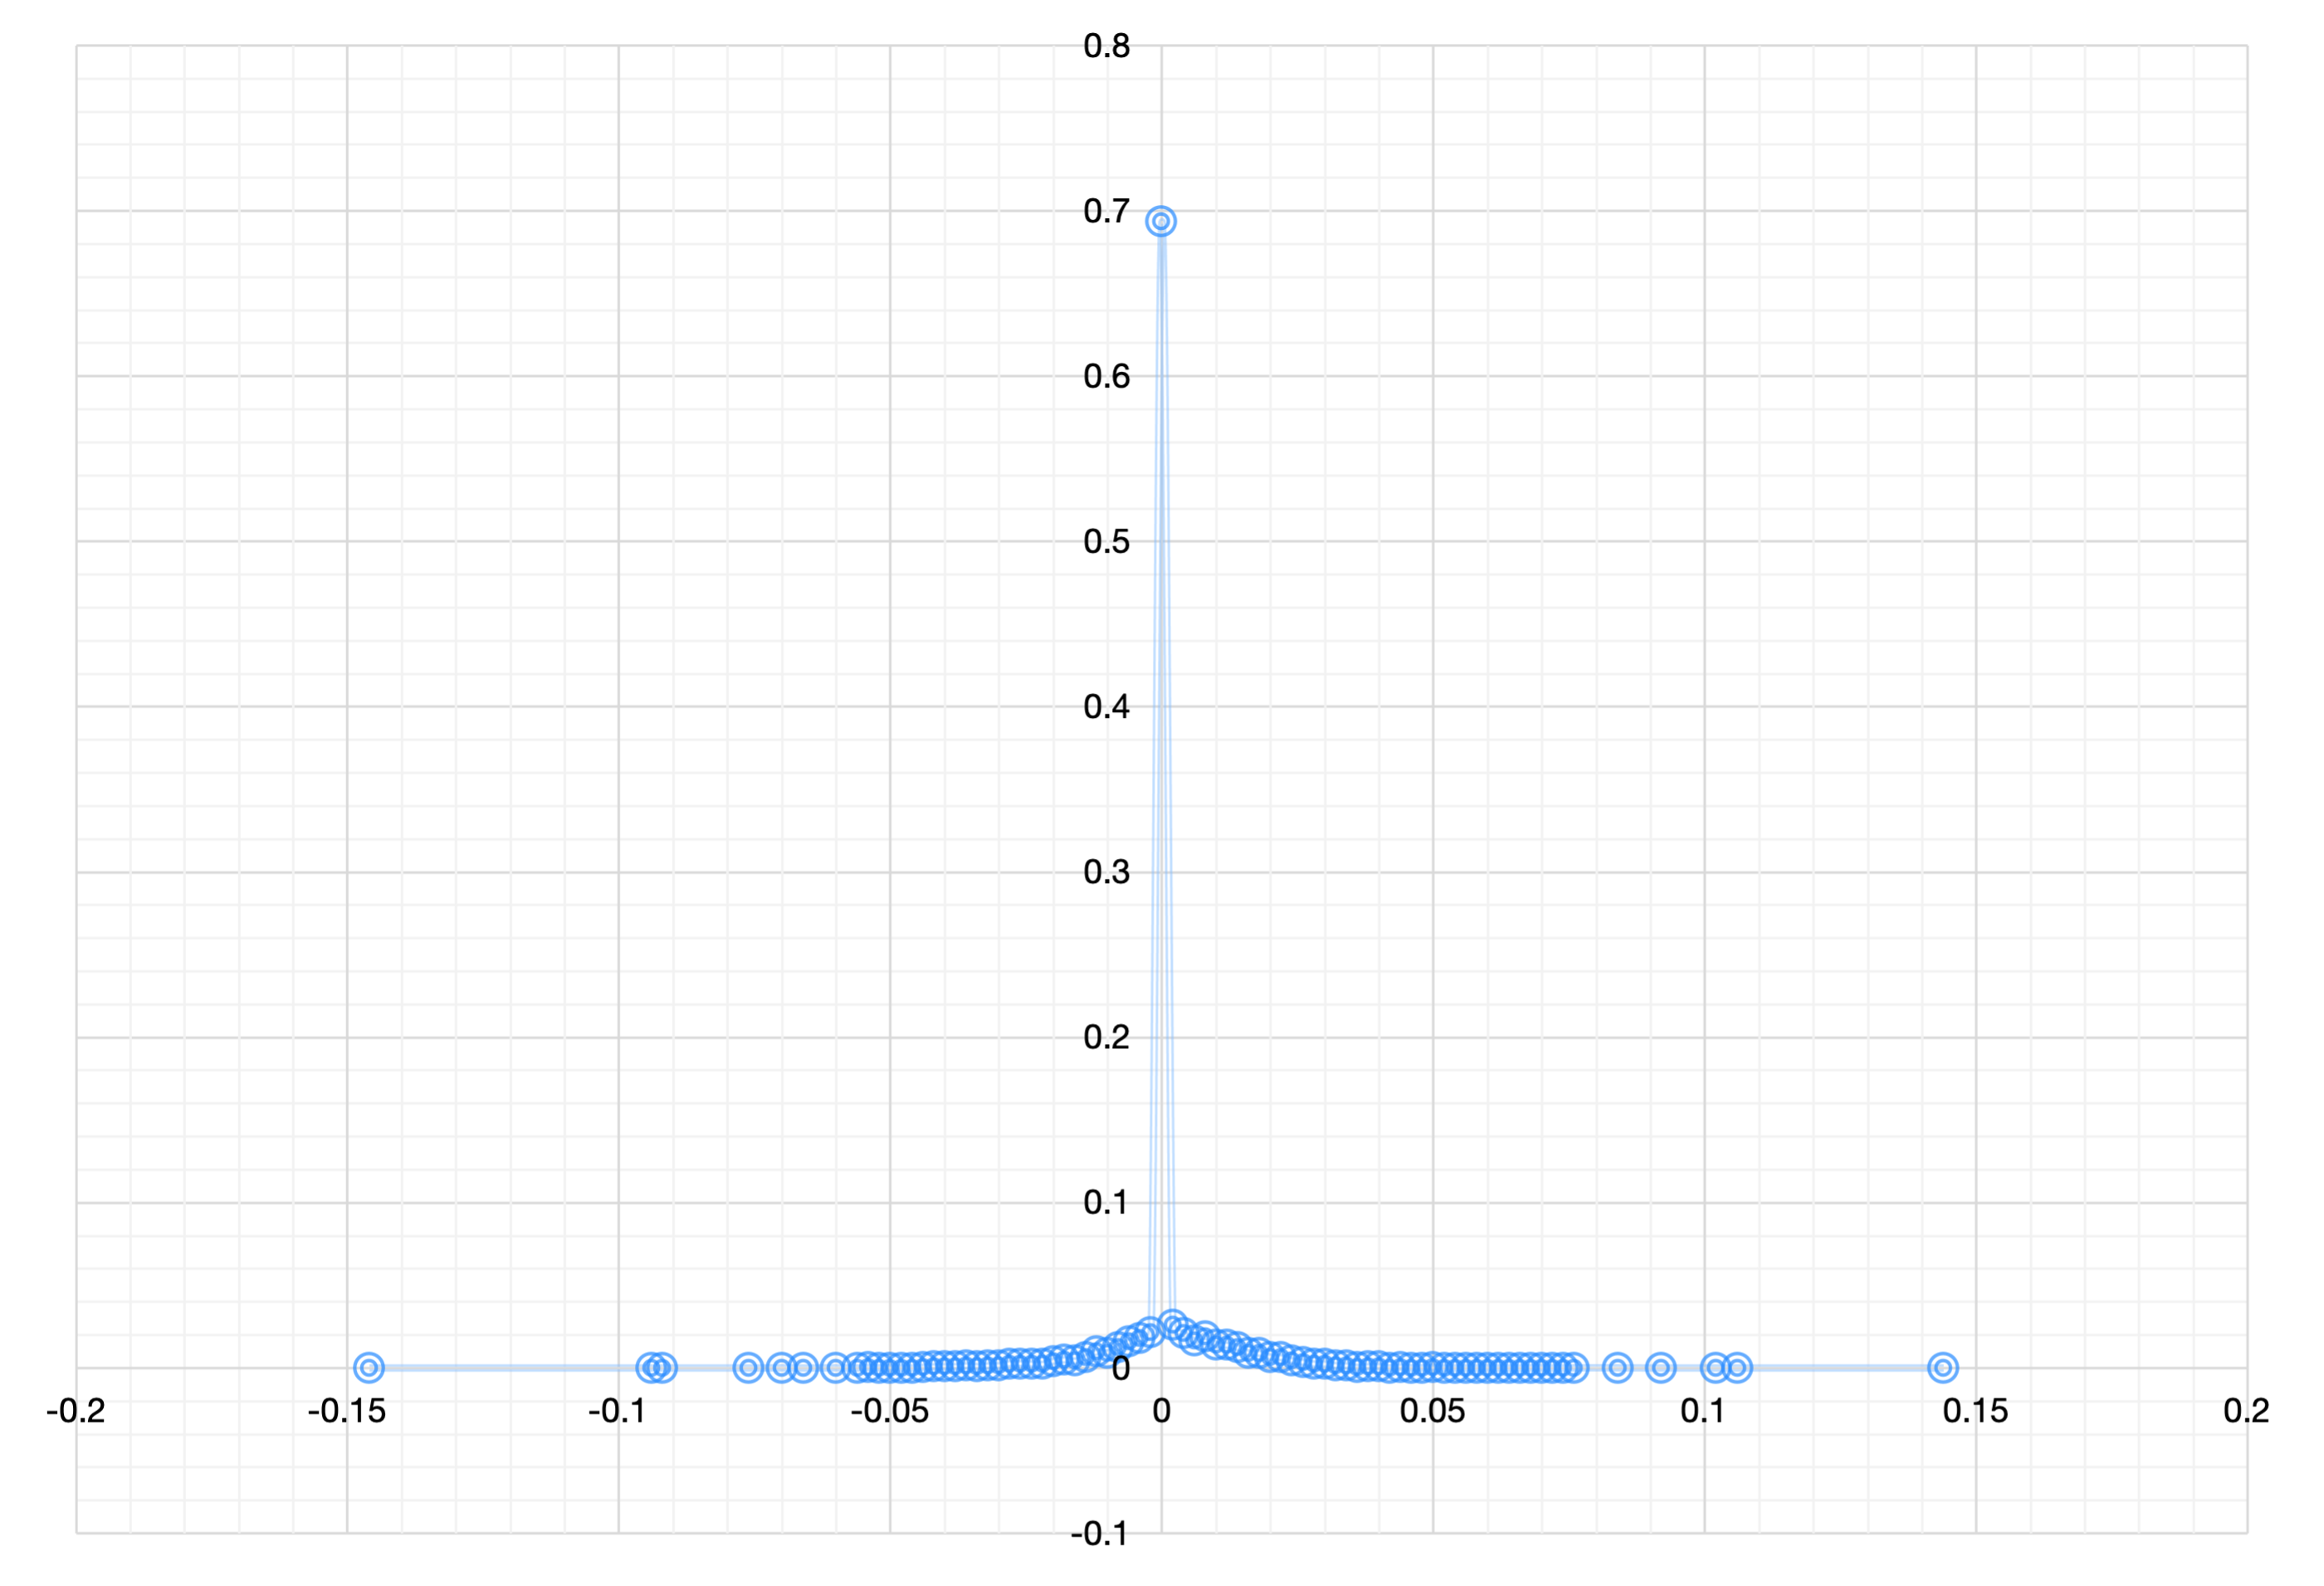
\includegraphics[width=0.5\textwidth]{HW1_Q7_1}
		   \end{figure}
	   
	   One notable thing we can see here is that there is an extremely high appearance of daily return as 0, as rounded up to 0.2\% interval. The total count is 5742, and corresponding probability is 0.693. This greatly distorts the plot.
	   
	   The we paste the value (without formula) into a new worksheet, and sort them with the ascending order of the unique counts, here we can calculate the cumulative probability using \texttt{=SUM(\$C\$2:C3)}, given column \texttt{C} is for single probability of each entry. Thus the cumulative distribution plot
	   
	   \pagebreak
	     \begin{figure}[h]
	     	\caption{Cumulative Distribution Function}
	     	\centering
	     	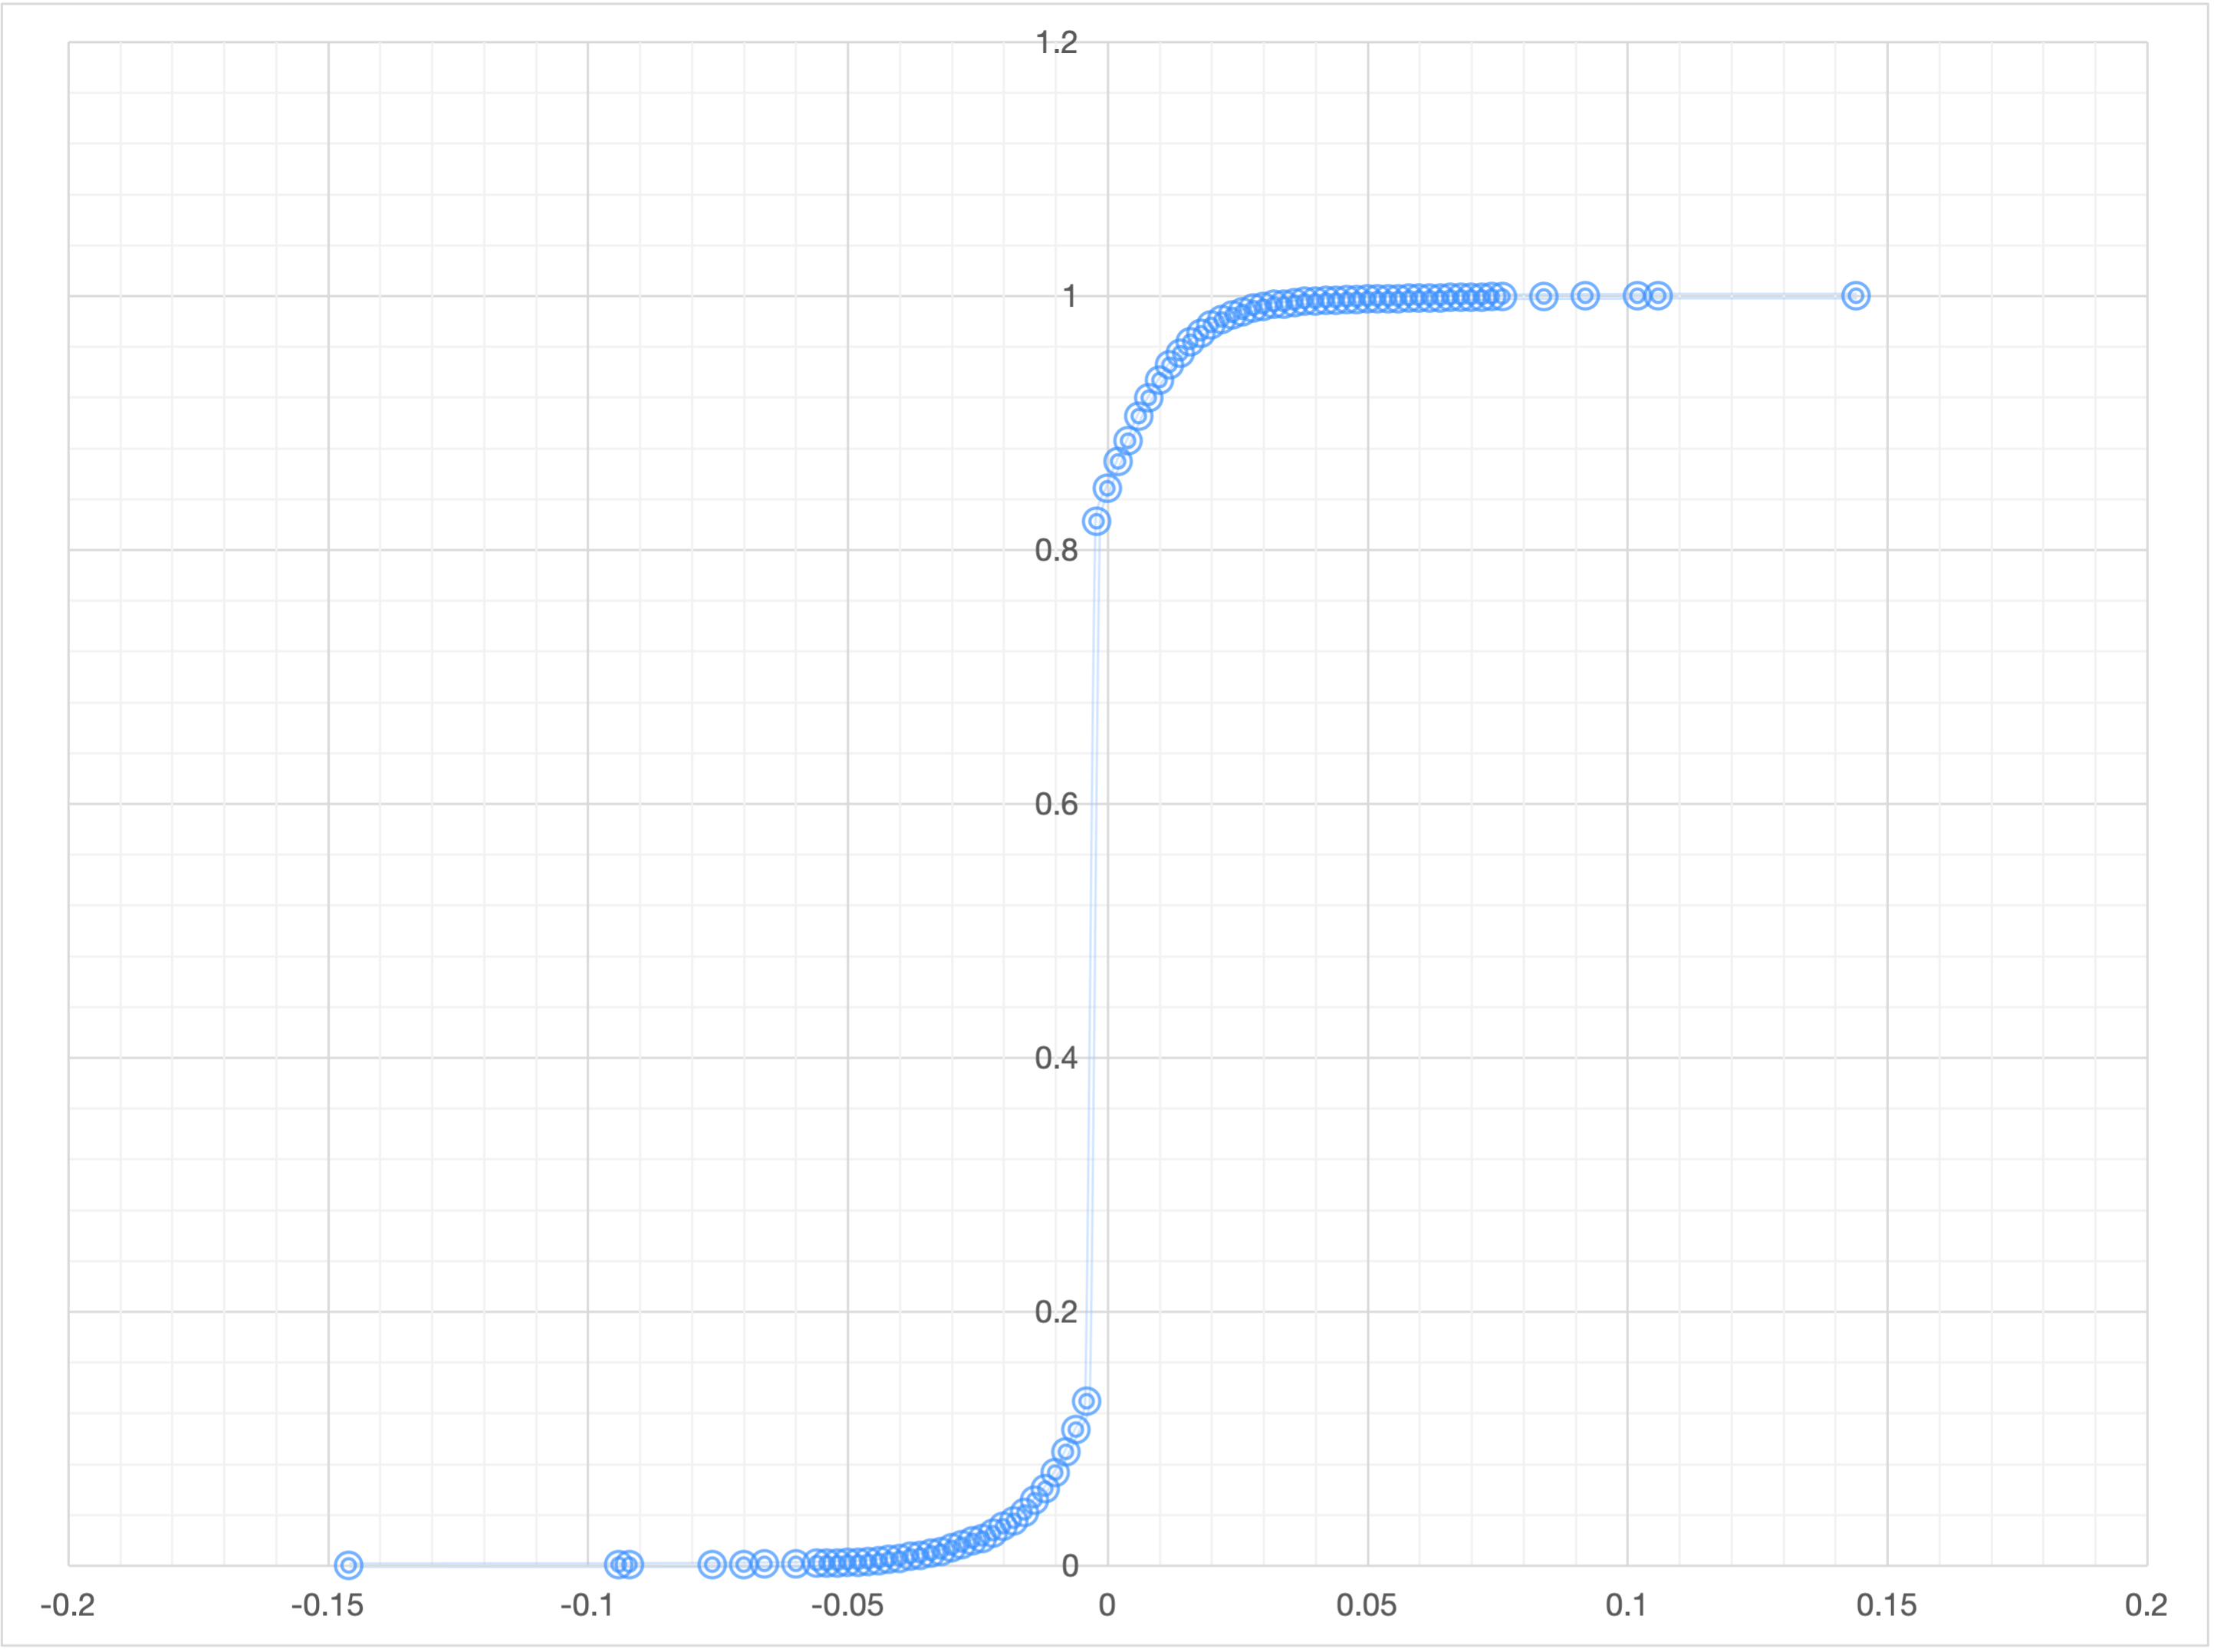
\includegraphics[width=0.5\textwidth]{HW1_Q7_2}
	     \end{figure}
		   
		   To calculate different measurements, I used functions provided by excel.
		   
		   \begin{itemize}
		   	\item For mean, I used \texttt{=AVERAGE(C:C)}, and the result is 0.001082704.
		   	\item For variance, I used \texttt{=VAR.P(C:C)}, and the result is 0.00027807.
		   	\item For standard deviation, I used \texttt{=STDEV.P(C:C)}, and the result is 0.01667544.
		   	\item For mean absolute deviation, I firstly used \texttt{=ABS(C2-\$G\$2)} to make a new column E, and then calculate the mean of this column with \texttt{=AVERAGE(E\$3:E\$1048576)}. And the result is 0.01146556.
		   	\item For kurtosis, I used \texttt{=KURT(C:C)}, and the result is 7.962253953.
		   	\item For skewness, I used \texttt{=SKEW(C:C)}, and the result is 0.077088852.
   			  \end{itemize}
	   
	   \pagebreak
		   
		   \subsubsection*{Question 8}
		   
		   \textbf{a} Calculate and plot 100 day, 50 day, 30 day and 15 day Moving Average of SPY Close from January 2, 2008 to January 15, 2025 in a spreadsheet similar to \texttt{HW1SPYMovingAve.xls}. Add data from Yahoo as needed. Submit printout of plots and last 20 days of data. 
		   
		   \textbf{b} Calculate and plot 15 day, 30 day, 50 day and 100 day volatility of SPY Adjusted Close from January 2, 2008 to January 15, 2025 in a spreadsheet similar to the \texttt{HW1SPYvol.xls}. Submit a printout.
		   
		   \textbf{Answer}
		   
		   In this question we need to download the SPY data from Yahoo and reorder it, to have its date from January 2, 2008 to January 15, 2025. Moreover, because it requires to calculate 100-day-volatile, which involves more data before year 2008, I also downloaded the data for year 2007 as well. 
		   
		   For question a, we have the Moving Average of SPY close for 100 day calculated as \texttt{=AVERAGE(E9:E108)}, for \texttt{E} is the close column. We can use this syntax for 50, 30, and 15 days, and the result is plotted as below:
		   \begin{figure}[h]
		   	\caption{Moving Average of SPY Close}
		   	\centering
		   	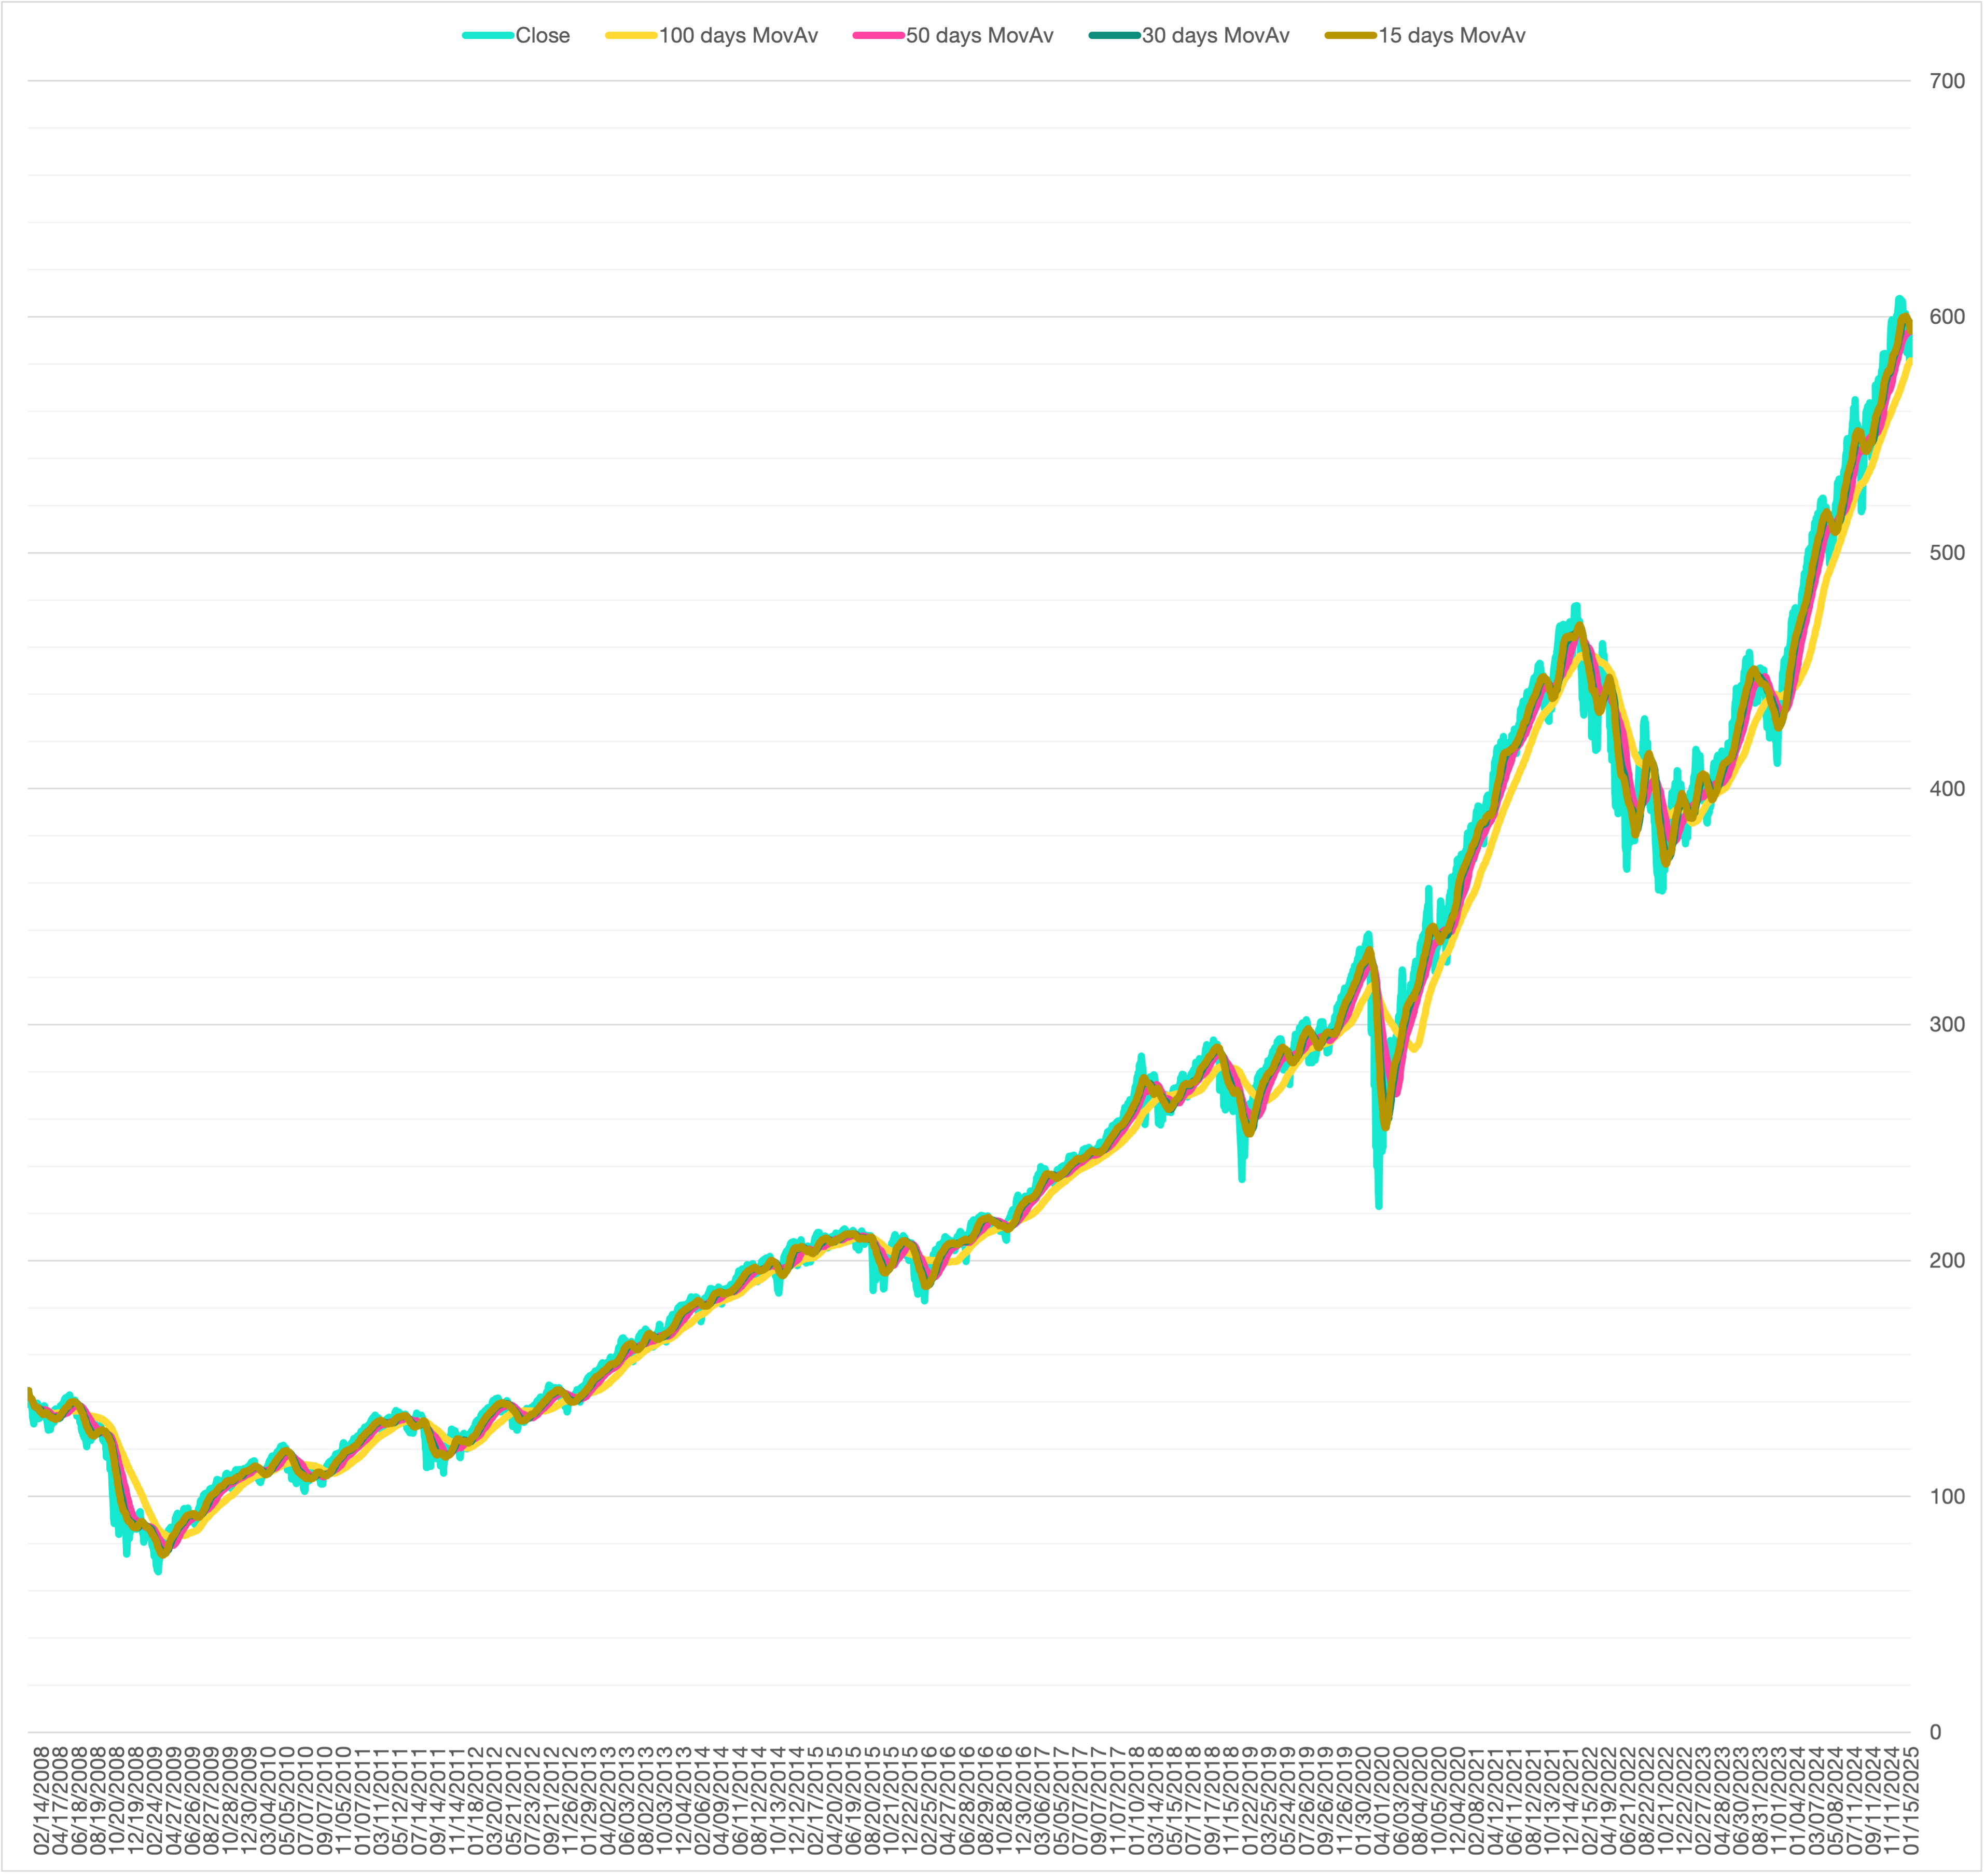
\includegraphics[width=0.6\textwidth]{HW1_Q8_1}
		   \end{figure}
	   
	   Moreover, I just double checked the rough chart in Yahoo Finance, and it gives a same plot. The red is an indicator for Moving Average.
	   
	   \begin{figure}[h]
	   	\caption{Moving Average of SPY Close for Yahoo Finance}
	   	\centering
	   	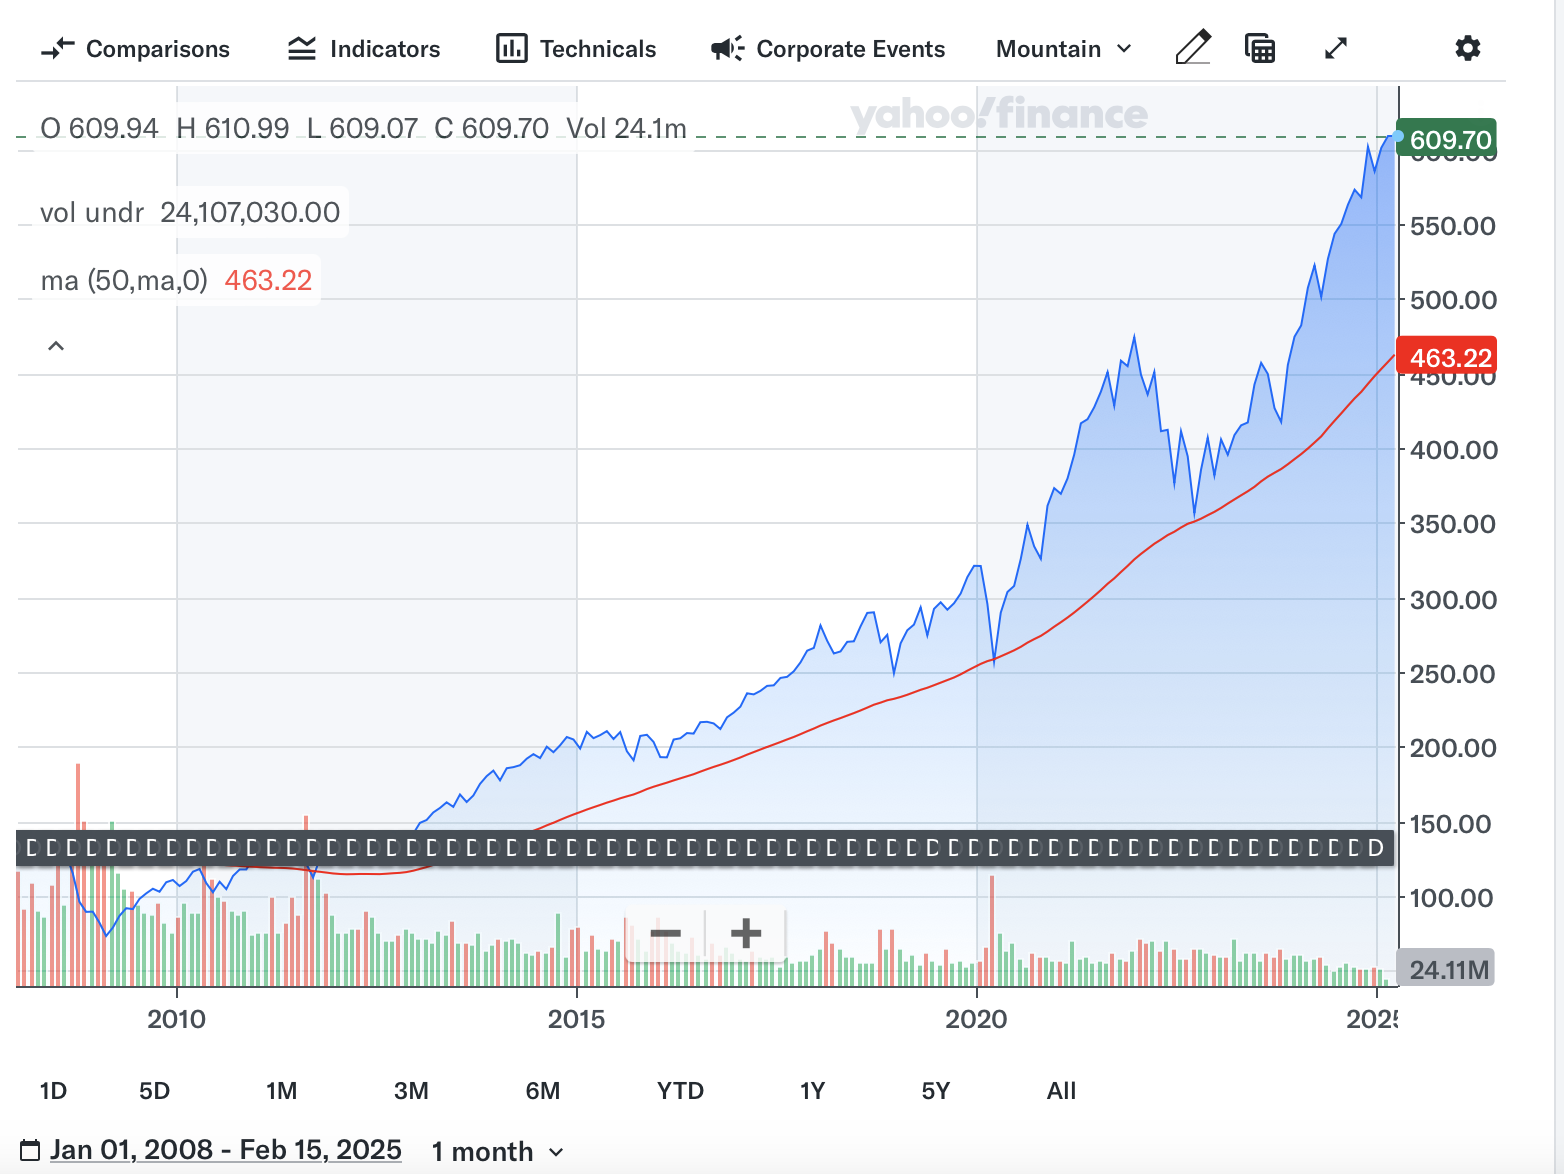
\includegraphics[width=0.7\textwidth]{HW1_Q8_1_1}
	   \end{figure}
	   
	   For question b, we first got the daily return in column \texttt{J}, and have the 100 day volatility calculated as \texttt{=STDEV(\$J9:\$J108)*SQRT(250)}, then have this applied for 15, 30, and 50 day volatility of SPY Adjusted Close. The result can be plotted as below:
		   \begin{figure}[h]
		   	\caption{Volatility of SPY Adjusted Close}
		   	\centering
		   	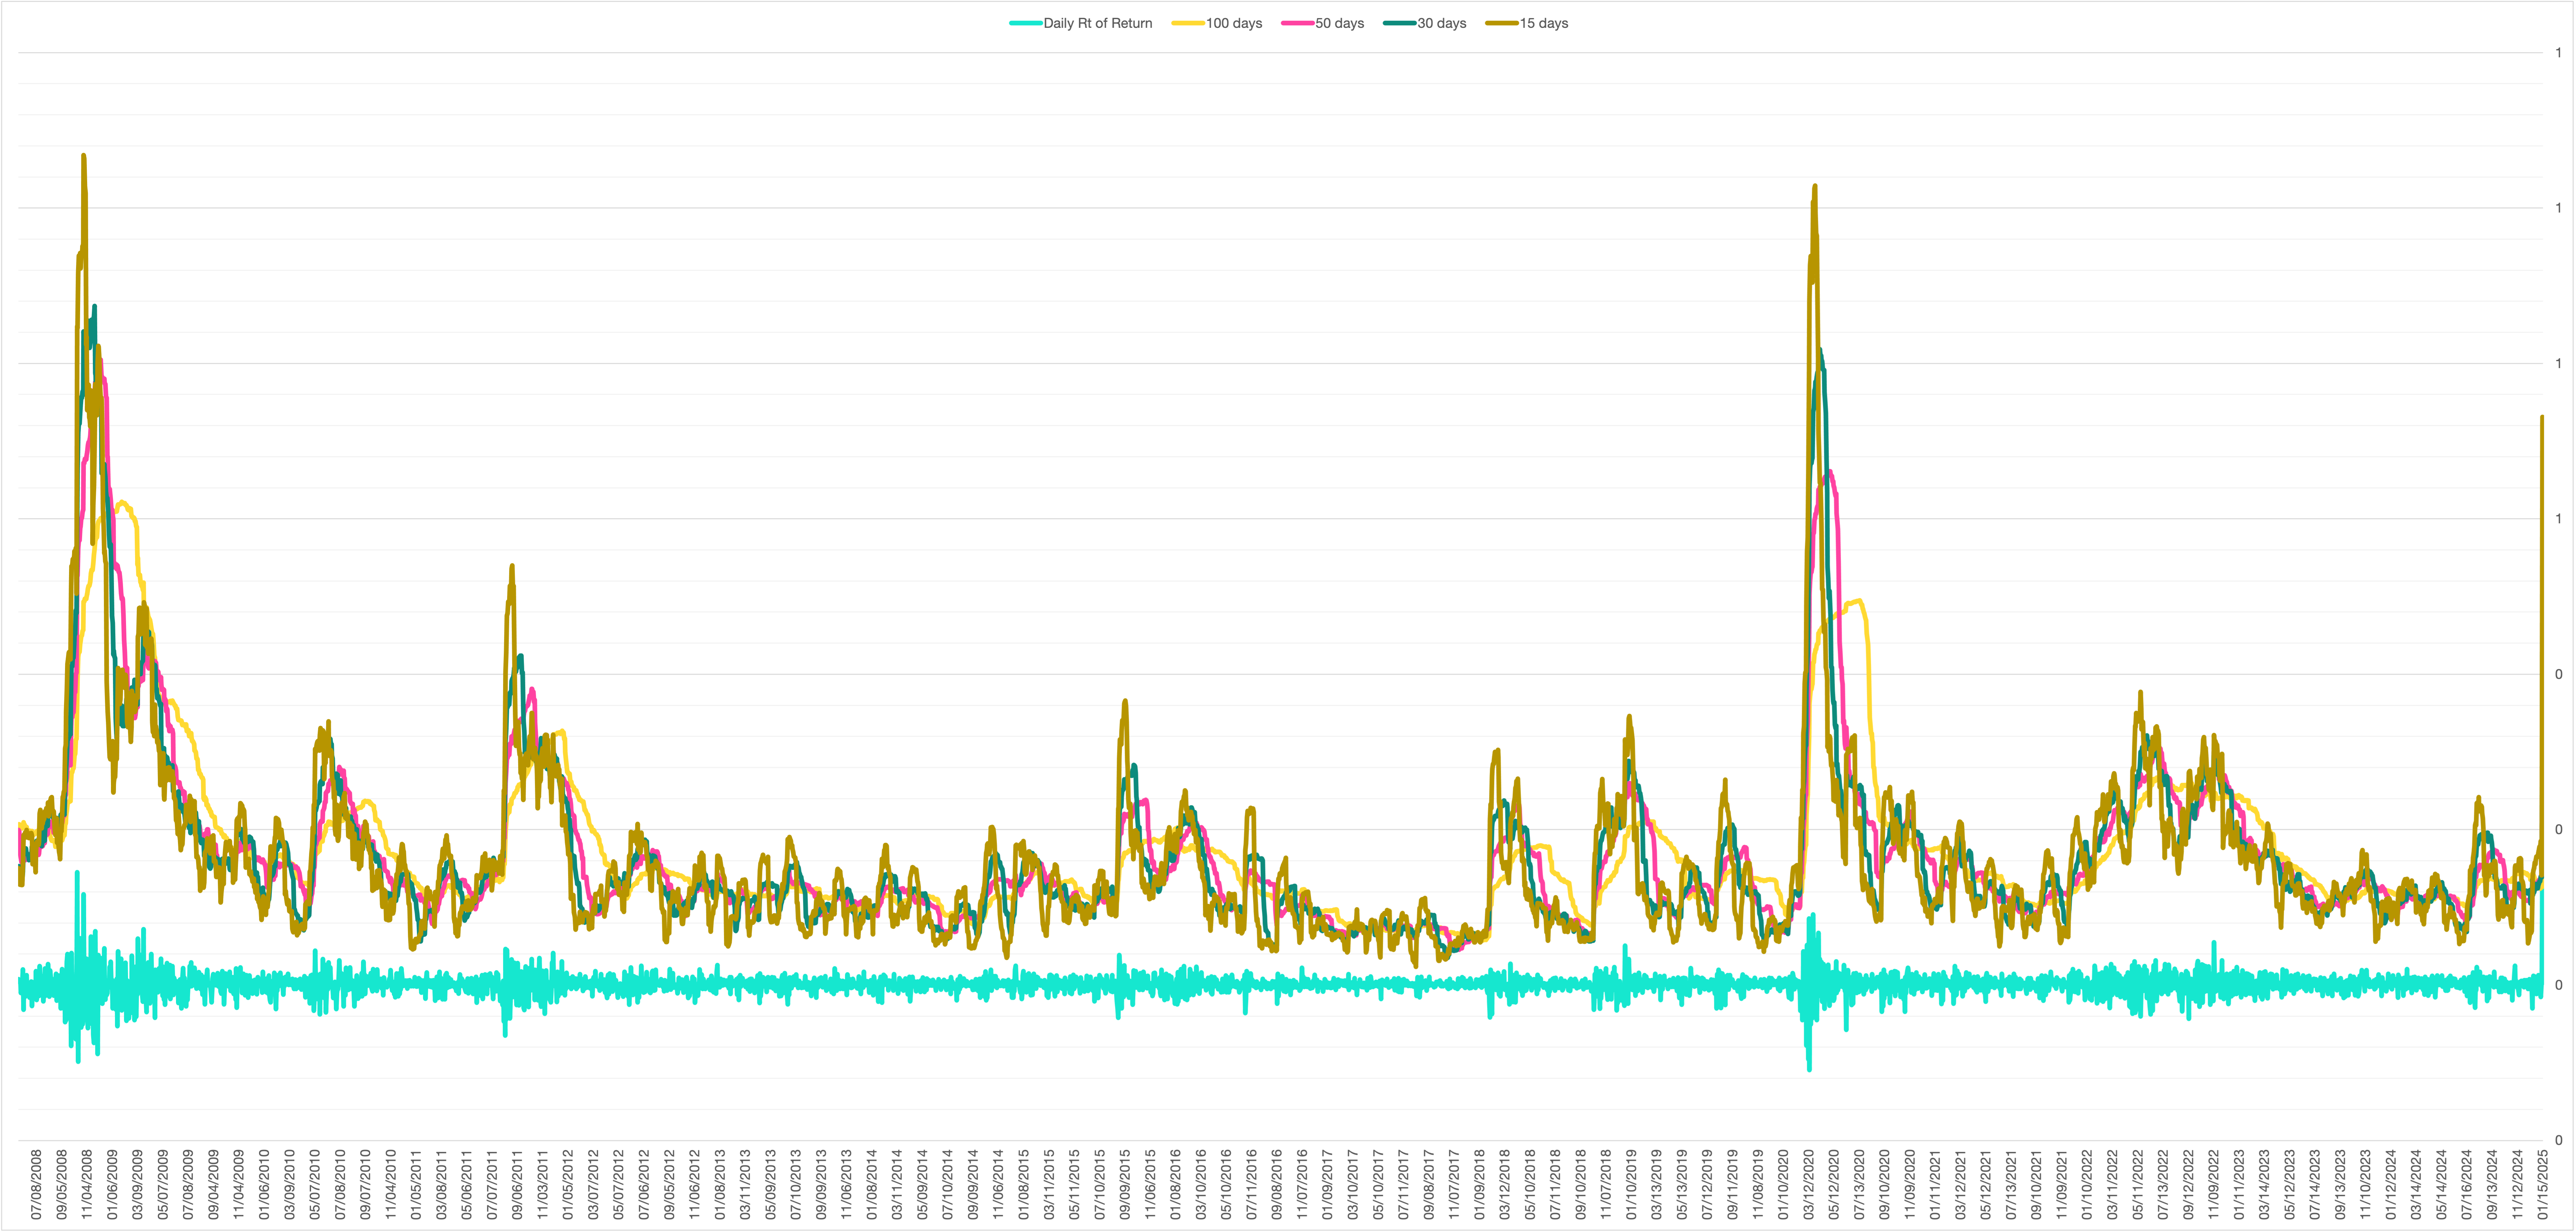
\includegraphics[width=0.7\textwidth]{HW1_Q8_2}
		   \end{figure}
		   
		   
		   \pagebreak
		   
		   \subsubsection*{Question 9}
		   Let X be a continuous random variable taking values between 0 and 4 with probability density function $\mathrm{p}(\mathrm{x})=$ 0.25. Find $E(X), \operatorname{Var}(X)$ and $\operatorname{Stdev}(X)$. Plot its Cumulative Distribution Function.
		  
		   \textbf{Answer}
		   
		   From the question, we can know that it is in fact a uniform distribution, thus I plotted it in R, with bins defined as 1000, to make it looks like a continuous function (it is, but adding too many bins would make hard fro computer to execute), the codes are as below:
		   

		   \begin{lstlisting}
		   	# Define the CDF function
		   	F_x <- function(x) {
		   		ifelse(x < 0, 0, ifelse(x > 4, 1, 0.25 * x))
		   	}
		   	
		   	# Generate x values
		   	x_vals <- seq(-1, 5, length.out = 1000)
		   	
		   	# Compute CDF values
		   	cdf_vals <- sapply(x_vals, F_x)
		   	
		   	# Plot the CDF
		   	plot(x_vals, cdf_vals, type="s", col="blue", lwd=2,
		   	xlab="x", ylab="F(x)", main="CDF of X ~ U(0,4)")
		   	abline(h=c(0,1), v=c(0,4), lty=2, col="red")
		   \end{lstlisting}
		   
		   It gives a plot like this
		   
		   \begin{figure}[h]
		   	\caption{Cumulative Distribution Function of  X $\sim$ U(0,4)}
		   	\centering
		   	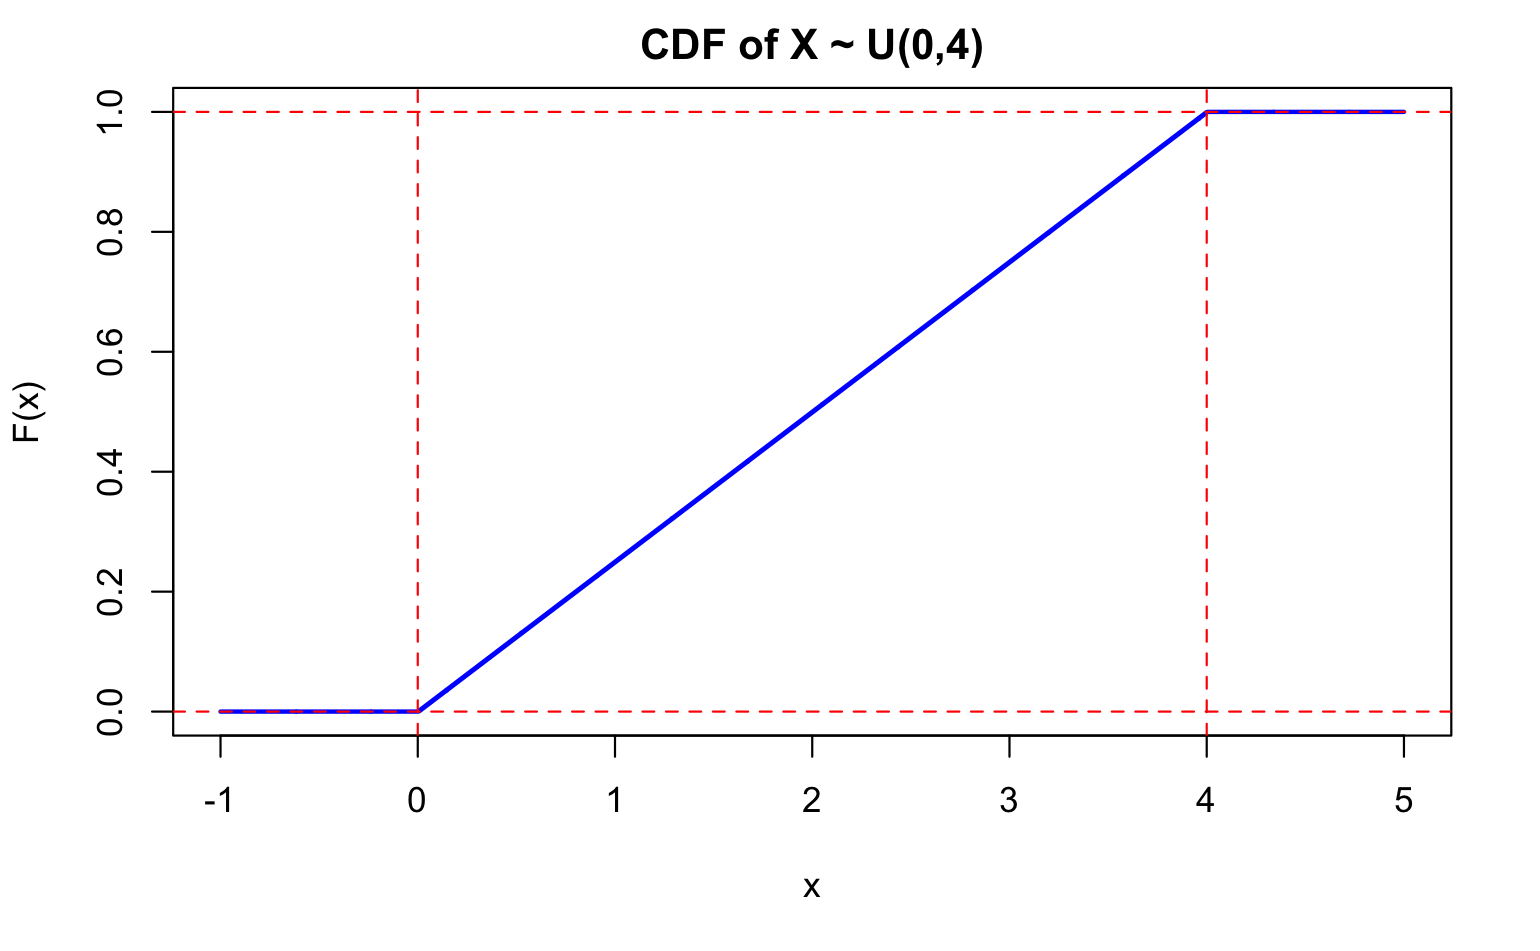
\includegraphics[width=0.7\textwidth]{HW1_Q9}
		   \end{figure}
	   
		   \pagebreak
		   
		   \subsubsection*{Question 10}
		   Suppose that $X$ and $Y$ are two normally distributed random variables. $X$ has mean 1 and standard deviation 2. Y has mean 4 and standard deviation 3 . Their correlation is 0.3 . What is the mean and standard deviation of $\mathrm{X}+\mathrm{Y}$ ? What is the distribution of $X+Y$ ? What if $X$ and $Y$ are jointly normally distributed? What if they are not jointly normally distributed? Explain your answer.
		   
		   \textbf{Answer}
		   
		   Supple that $x$ and $y$ are two normally distributed random variables. $x$ has mean 1 and standard deviation 2. y has mean 4 and standard deviation 3.
		   $$
		   \begin{aligned}
		   	& x \sim N(\mu=1, \sigma=2) \sim N\left(1,2^2\right) \\
		   	& y \sim N(\mu=4, \sigma=3) \sim N\left(4,3^2\right) \\
		   	& \text { correlation is } \rho=0.3
		   \end{aligned}
		   $$
		   
		   The sum of two normally distributed random variables are also normally distributed. Thus $X+Y$ is a normal distribution.
		   
		   Suppose $x$ and $y$ are jointly normally distributed:
		   $$
		   \begin{aligned}
		   	x+y \longrightarrow N & \left(\mu_x+\mu_y, \sigma_x^2+\sigma y^2+2 \rho \sigma_x \sigma_y\right) \\
		   	\mu_x+\mu_y & =1+4 \\
		   	& =5 \\
		   	\sigma x^2+\sigma y^2+2 \rho \sigma_x \sigma_y & =2^2+3^2+2(0.3)(2 \times 3) \\
		   	& =4+9+2(0.3)(6) \\
		   	& =16.6\\
		   	& x+y \rightarrow N(5,16.6) \\
		   	& x+y \rightarrow N\left(\mu=5, \rho^2=16.6\right) \\
		   	& \text{Thus the standard deviation is} \sqrt{16.6} \approx 4.08
		\end{aligned}
	$$
		   
		   Suppose they are not jointly normally distributed, we can only say that mean is 5 and standard deviation is 4.08, for the new function $X+Y$, yet we can not know is the new distribution is normal.
		   
		   	
		   \subsubsection*{Question 11}
		   Suppose you are applying to graduate schools. Your chances to be admitted to each one school are $10 \%$ and are the same for any school. To how many different schools you need to apply if you want your chances to be admitted to at least one school to be above 95\%.
		   
		   \textbf{Answer}
		   
		   In the question, we can get the information
		   $$
		   \begin{aligned}
		   	& 1-0.1=0.9\\
		   	& 1-0.9^{n}>0.95\\
		   	& 0.9^{n}<0.05\\
		   	& n>\frac{ln(0.05)}{ln(0.9)}=28.433
		   \end{aligned}
	   $$
	   
	   Rounding up, we should apply to 29 different schools  if we want the chances to be admitted to at least one school to be above 95%
		
		
	\pagebreak
	 
	\end{document}